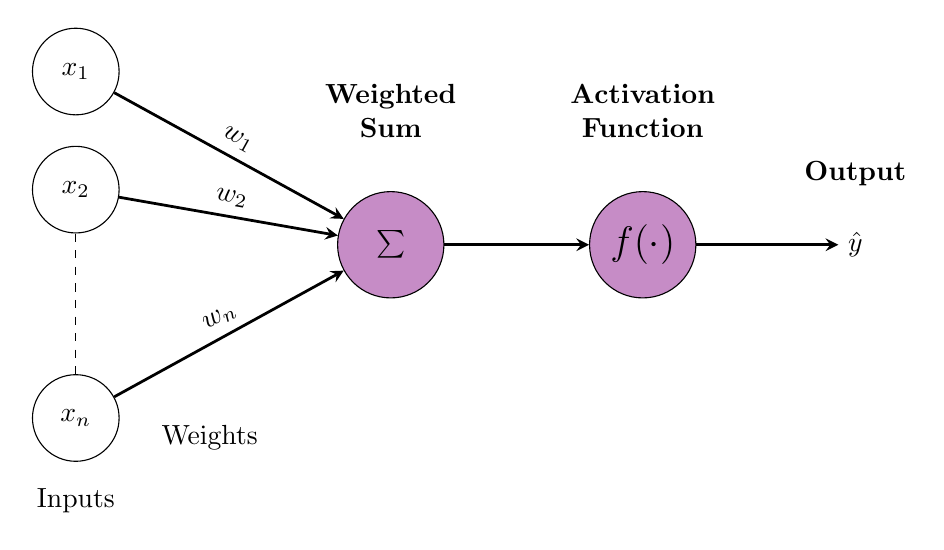
\begin{tikzpicture}[
    node distance=1.8cm,
    neuron/.style={circle, draw, minimum size=1.1cm, font=\bfseries},
    block/.style={circle, draw, fill=violet!45, minimum size=1.35cm},
    arrow/.style={->, >=stealth, line width=1pt},
    label/.style={font=\bfseries}
]

% Inputs
\node[neuron] (x1) at (0,2.2) {$x_1$};
\node[neuron] (x2) at (0,0.7) {$x_2$};
\node[neuron] (xn) at (0,-2.2) {$x_n$};

\draw[dashed] (x2) -- (xn);

\node at (0,-3.25) {Inputs};

% Weighted sum
\node[block] (sum) at (4,0) {\Large $\sum$};
\node[label, align=center] at (4,1.7) {Weighted\\Sum};

% Activation function
\node[block] (act) at (7.2,0) {\Large $f(\cdot)$};
\node[label, align=center] at (7.2,1.7) {Activation\\Function};

% Output
\node[label] (outlabel) at (9.9,0.9) {Output};
\node (out) at (9.9,0) {$\hat{y}$};

% Arrows from inputs
\draw[arrow] (x1) -- node[above, sloped] {$w_1$} (sum);
\draw[arrow] (x2) -- node[above, sloped] {$w_2$} (sum);
\draw[arrow] (xn) -- node[above, sloped] {$w_n$} (sum);

% Arrows between processing nodes
\draw[arrow] (sum) -- (act);
\draw[arrow] (act) -- (out);

% Weights label
\node at (1.7,-2.45) {Weights};

\end{tikzpicture}